\documentclass[9pt,a4paper]{extarticle}
\usepackage[margin=1.2cm]{geometry}
\usepackage{multicol}
\usepackage{amsmath,amssymb}
\usepackage{mathtools}
\usepackage{xcolor}
\usepackage{tikz}
\usepackage{pgfplots}
\pgfplotsset{compat=1.18}
\usepackage{tcolorbox}
\tcbuselibrary{skins,breakable}
\usepackage{listings}
\usepackage{fancyhdr}
\usepackage{array,booktabs,tabularx}
\usepackage{enumitem}
\usepackage{microtype}
\usetikzlibrary{arrows.meta,positioning,shapes.geometric,calc,backgrounds}

\definecolor{pytorchred}{HTML}{EE4C2C}
\definecolor{deepblue}{HTML}{1A237E}
\definecolor{codeblue}{HTML}{1565C0}
\definecolor{mathgreen}{HTML}{1B5E20}
\definecolor{warnorange}{HTML}{E65100}
\definecolor{bgcode}{HTML}{FAFAFA}
\definecolor{accentpurple}{HTML}{4A148C}
\definecolor{tealcolor}{HTML}{006064}
\definecolor{noteyellow}{HTML}{FFF8E1}
\definecolor{defblue}{HTML}{E3F2FD}
\definecolor{tipgreen}{HTML}{E8F5E9}
\definecolor{warnred}{HTML}{FFEBEE}
\definecolor{darkgray}{HTML}{263238}

\lstdefinestyle{pytorch}{
  language=Python,
  basicstyle=\ttfamily\fontsize{6.5pt}{8pt}\selectfont,
  keywordstyle=\color{codeblue}\bfseries,
  commentstyle=\color{gray}\itshape,
  stringstyle=\color{pytorchred},
  backgroundcolor=\color{bgcode},
  frame=single,framerule=0.4pt,rulecolor=\color{gray!40},
  breaklines=true,tabsize=2,showstringspaces=false,
  xleftmargin=4pt,xrightmargin=4pt,aboveskip=2pt,belowskip=2pt,
  morekeywords={torch,nn,optim,DataLoader,Dataset}
}
\lstset{style=pytorch}

\tcbset{
  defbox/.style={colback=defblue,colframe=codeblue,fonttitle=\bfseries\small,coltitle=white,arc=3pt,boxrule=0.6pt,top=3pt,bottom=3pt,left=4pt,right=4pt,toptitle=1.5pt,bottomtitle=1.5pt},
  mathbox/.style={colback=tipgreen,colframe=mathgreen,fonttitle=\bfseries\small,coltitle=white,arc=3pt,boxrule=0.6pt,top=3pt,bottom=3pt,left=4pt,right=4pt,toptitle=1.5pt,bottomtitle=1.5pt},
  warnbox/.style={colback=warnred,colframe=pytorchred,fonttitle=\bfseries\small,coltitle=white,arc=3pt,boxrule=0.6pt,top=3pt,bottom=3pt,left=4pt,right=4pt,toptitle=1.5pt,bottomtitle=1.5pt},
  tipbox/.style={colback=noteyellow,colframe=warnorange,fonttitle=\bfseries\small,coltitle=white,arc=3pt,boxrule=0.6pt,top=3pt,bottom=3pt,left=4pt,right=4pt,toptitle=1.5pt,bottomtitle=1.5pt}
}

\newcommand{\mysec}[2]{\vspace{3pt}\noindent\colorbox{#1}{\parbox{\linewidth-2\fboxsep}{\color{white}\bfseries\fontsize{8pt}{10pt}\selectfont\hspace{2pt}#2}}\vspace{2pt}}
\newcommand{\mysubsec}[1]{\vspace{2pt}\noindent{\color{deepblue}\fontsize{7.5pt}{9pt}\selectfont\bfseries\rule[-.5ex]{0.25em}{1.2ex}\hspace{3pt}#1}\vspace{1pt}}

\pagestyle{fancy}
\fancyhf{}
\renewcommand{\headrulewidth}{1pt}
\renewcommand{\headrule}{\hbox to\headwidth{\color{pytorchred}\leaders\hrule height\headrulewidth\hfill}}
\fancyhead[L]{\color{pytorchred}\bfseries\small PyTorch 3-Hour Lock-In Study Sheet}
\fancyhead[R]{\color{darkgray}\small\bfseries Deep Learning Fundamentals}
\fancyfoot[C]{\color{gray}\small Page \thepage\ of 6}
\fancyfoot[R]{\color{gray}\tiny torch | autograd | nn | optim}

\setlength{\columnsep}{8pt}
\setlength{\columnseprule}{0.3pt}
\setlist[itemize]{noitemsep,topsep=1pt,leftmargin=10pt,label=\textcolor{pytorchred}{\tiny\textbullet}}
\setlist[enumerate]{noitemsep,topsep=1pt,leftmargin=12pt}
\parindent=0pt
\parskip=1.5pt

\begin{document}

%%%% PAGE 1 - TENSORS %%%%
\begin{multicols}{3}

\mysec{pytorchred}{WHAT IS PYTORCH?}

\begin{tcolorbox}[defbox,title=Definition]
\fontsize{7pt}{9pt}\selectfont
PyTorch is an open-source deep learning framework by Meta AI providing:\\
\textbf{(1)} N-dimensional tensor computation (GPU NumPy)\\
\textbf{(2)} Automatic differentiation (\texttt{autograd})\\
\textbf{(3)} Dynamic computation graph (Define-by-Run)
\end{tcolorbox}

\begin{tcolorbox}[tipbox,title=Why Dynamic Graph?]
\fontsize{7pt}{9pt}\selectfont
Graph built \textit{on the fly} during execution. Use normal Python \texttt{if/else}, \texttt{print()}, \texttt{pdb} directly on models. TF1.x used static graphs --- harder to debug.
\end{tcolorbox}

\mysec{deepblue}{TENSOR --- THE DNA}

\begin{tcolorbox}[defbox,title=Definition]
\fontsize{7pt}{9pt}\selectfont
A \textbf{Tensor} is a generalized multi-dimensional array unifying scalars, vectors, and matrices under one structure.
\end{tcolorbox}

\mysubsec{Tensor Dimensionality}

{\fontsize{6.5pt}{8pt}\selectfont
\renewcommand{\arraystretch}{1.2}
\begin{tabular}{@{}cccl@{}}
\toprule
\textbf{Name}&\textbf{Dim}&\textbf{Notation}&\textbf{Example}\\
\midrule
Scalar&0D&$x\in\mathbb{R}$&$5$\\
Vector&1D&$\mathbf{x}\in\mathbb{R}^n$&$[1,2,3]$\\
Matrix&2D&$\mathbf{X}\in\mathbb{R}^{m\times n}$&grid\\
3D Tensor&3D&$\mathcal{T}\in\mathbb{R}^{d\times m\times n}$&RGB image\\
4D Tensor&4D&$\mathcal{T}\in\mathbb{R}^{B\times C\times H\times W}$&batch\\
\bottomrule
\end{tabular}}

\begin{center}
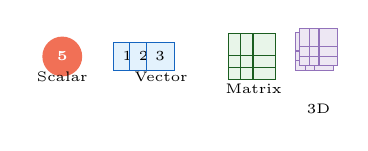
\begin{tikzpicture}[scale=0.55]
  \node[circle,fill=pytorchred!80,text=white,minimum size=14pt,font=\tiny\bfseries] at (0,0) {5};
  \node[font=\tiny,below=2pt] at (0,0) {Scalar};
  \foreach \i/\v in {0/1,1/2,2/3}{
    \node[draw=codeblue,fill=defblue,minimum width=10pt,minimum height=10pt,font=\tiny] at (1.5+\i*0.38,0) {\v};
  }
  \node[font=\tiny,below=2pt] at (2.28,0) {Vector};
  \foreach \r in {0,1,2}{
    \foreach \c in {0,1,2}{
      \node[draw=mathgreen,fill=tipgreen,minimum width=8pt,minimum height=8pt] at (4.1+\c*0.28,\r*0.28-0.28) {};
    }
  }
  \node[font=\tiny,below=2pt] at (4.42,-0.28) {Matrix};
  \begin{scope}[shift={(5.6,-0.1)}]
    \foreach \d in {0,1}{
      \foreach \r in {0,1,2}{
        \foreach \c in {0,1,2}{
          \node[draw=accentpurple!60,fill=accentpurple!10,minimum width=6pt,minimum height=6pt] at (\c*0.22+\d*0.10,\r*0.22+\d*0.10) {};
        }
      }
    }
    \node[font=\tiny,below=12pt] at (0.32,0) {3D};
  \end{scope}
\end{tikzpicture}
\end{center}

\mysubsec{Batch Image Shape}

$\mathcal{T}\in\mathbb{R}^{B\times C\times H\times W}$: $B{=}32$ (batch), $C{=}3$ (RGB), $H,W{=}224$

\mysec{tealcolor}{CREATING TENSORS}

{\fontsize{6.5pt}{8pt}\selectfont
\renewcommand{\arraystretch}{1.15}
\begin{tabularx}{\linewidth}{@{}lX@{}}
\toprule
\textbf{Syntax}&\textbf{Purpose}\\
\midrule
\lstinline|torch.tensor([1,2,3])|&From Python list\\
\lstinline|torch.zeros(3,4)|&All zeros\\
\lstinline|torch.ones(3,4)|&All ones\\
\lstinline|torch.rand(3,4)|&Uniform $\mathcal{U}[0,1)$\\
\lstinline|torch.randn(3,4)|&Normal $\mathcal{N}(0,1)$\\
\lstinline|torch.arange(0,10,2)|&Integer range\\
\lstinline|torch.linspace(0,1,5)|&Evenly spaced\\
\lstinline|torch.eye(3)|&Identity $\mathbf{I}_3$\\
\lstinline|torch.zeros_like(t)|&Same shape, zeros\\
\lstinline|torch.empty(2,3)|&Uninitialized\\
\bottomrule
\end{tabularx}}

\begin{tcolorbox}[warnbox,title=Key Distinction]
\fontsize{7pt}{9pt}\selectfont
\texttt{torch.tensor()} \textbf{copies} data.\\
\texttt{torch.as\_tensor()} \textbf{shares} memory with NumPy arrays.
\end{tcolorbox}

\mysec{accentpurple}{TENSOR ATTRIBUTES (BIG THREE)}

\begin{tcolorbox}[mathbox,title=Three Core Properties]
\fontsize{7pt}{9pt}\selectfont
\texttt{t.dtype} \hfill data type stored\\
\texttt{t.shape} \hfill dimensions (torch.Size)\\
\texttt{t.device} \hfill cpu / cuda / mps\\[2pt]
Also: \texttt{t.ndim}, \texttt{t.numel()}
\end{tcolorbox}

{\fontsize{6.5pt}{8pt}\selectfont
\begin{tabular}{@{}ll@{}}
\toprule
\textbf{dtype}&\textbf{Use}\\
\midrule
\texttt{float32}&Default NN weights\\
\texttt{float16}&GPU half-precision\\
\texttt{int64}&Default integers\\
\texttt{bool}&Masks, conditions\\
\bottomrule
\end{tabular}}

\mysec{pytorchred}{DEVICE MANAGEMENT}

\begin{lstlisting}
device = "cuda" if torch.cuda.is_available() else "cpu"
t = t.to(device)    # move tensor
t = t.cuda()        # shorthand GPU
t = t.cpu()         # back to CPU
\end{lstlisting}

\begin{tcolorbox}[warnbox,title=Common Error]
\fontsize{7pt}{9pt}\selectfont
Two tensors must be on \textbf{same device}. Mixing cpu/cuda throws \texttt{RuntimeError}. Move \textit{both} model \textbf{and} data!
\end{tcolorbox}

\mysec{deepblue}{TENSOR OPERATIONS}

\mysubsec{Element-wise}

{\fontsize{6.5pt}{8pt}\selectfont
$(a\odot b)_{ij}=a_{ij}\cdot b_{ij}$ --- operates at each position independently}

\begin{lstlisting}
a*b; a+b; a-b; a/b
torch.sqrt(a); torch.exp(a); torch.log(a)
\end{lstlisting}

\mysubsec{Matrix Multiplication --- MOST IMPORTANT}

For $\mathbf{A}\in\mathbb{R}^{m\times n}$, $\mathbf{B}\in\mathbb{R}^{n\times p}$:

\begin{tcolorbox}[mathbox]
\fontsize{8pt}{11pt}\selectfont
\vspace{-3pt}
\[
\mathbf{C}=\mathbf{AB}\in\mathbb{R}^{m\times p},\quad C_{ij}=\sum_{k=1}^{n}A_{ik}B_{kj}
\]
\vspace{-5pt}
\end{tcolorbox}

\begin{lstlisting}
A @ B              # preferred (batched too)
torch.matmul(A,B)  # same
torch.mm(A,B)      # 2D only
\end{lstlisting}

\begin{tcolorbox}[warnbox]
\fontsize{7pt}{9pt}\selectfont
\texttt{a * b} = element-wise \quad\quad \texttt{a @ b} = matmul
\end{tcolorbox}

\mysubsec{Aggregation}

\begin{lstlisting}
t.sum(); t.mean(); t.std()
t.max(); t.argmax(); t.argmin()
t.sum(dim=0)   # collapse rows
t.sum(dim=1)   # collapse columns
\end{lstlisting}

{\fontsize{7pt}{9pt}\selectfont
$\mu=\dfrac{1}{n}\sum_{i}x_i$ \qquad $\sigma=\sqrt{\dfrac{1}{n}\sum_{i}(x_i-\mu)^2}$}

\end{multicols}

%%%% PAGE 2 - SHAPES + AUTOGRAD %%%%
\newpage
\begin{multicols}{3}

\mysec{tealcolor}{SHAPE MANIPULATION}

{\fontsize{6.5pt}{8pt}\selectfont
\renewcommand{\arraystretch}{1.15}
\begin{tabularx}{\linewidth}{@{}lX@{}}
\toprule
\textbf{Operation}&\textbf{Effect}\\
\midrule
\texttt{reshape(r,c)}&New shape, may copy\\
\texttt{view(r,c)}&New shape, shares mem\\
\texttt{squeeze()}&Remove size-1 dims\\
\texttt{unsqueeze(0)}&Add dim at pos 0\\
\texttt{permute(2,0,1)}&Reorder all dims\\
\texttt{transpose(0,1)}&Swap two dims\\
\texttt{flatten()}&Collapse to 1D\\
\texttt{cat([a,b],dim=0)}&Concat existing dim\\
\texttt{stack([a,b],dim=0)}&Create new dim\\
\bottomrule
\end{tabularx}}

\begin{tcolorbox}[tipbox,title=The -1 Trick]
\fontsize{7pt}{9pt}\selectfont
\texttt{t.reshape(32,-1)}: PyTorch infers the second dim. If $t$ has $32{\times}N$ elements, result is $(32,N)$.
\end{tcolorbox}

\begin{tcolorbox}[warnbox,title=PIL vs PyTorch Format]
\fontsize{7pt}{9pt}\selectfont
PIL/NumPy: $(H,W,C)$\\
PyTorch: $(C,H,W)$\\
Convert: \texttt{tensor.permute(2,0,1)}
\end{tcolorbox}

\begin{center}
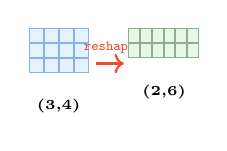
\begin{tikzpicture}[scale=0.6,font=\tiny]
  \foreach \r in {0,1,2}{
    \foreach \c in {0,1,2,3}{
      \fill[defblue,draw=codeblue!50,line width=0.3pt] (\c*0.32,-\r*0.32) rectangle (\c*0.32+0.30,-\r*0.32+0.30);
    }
  }
  \node[below,font=\fontsize{5pt}{6pt}\selectfont] at (0.62,-1.0) {\textbf{(3,4)}};
  \draw[->,thick,pytorchred] (1.4,-0.45)--node[above,font=\fontsize{5pt}{6pt}\selectfont]{\texttt{reshape}}(2.0,-0.45);
  \foreach \r in {0,1}{
    \foreach \c in {0,...,5}{
      \fill[tipgreen,draw=mathgreen!50,line width=0.3pt] (2.1+\c*0.25,-\r*0.32) rectangle (2.1+\c*0.25+0.23,-\r*0.32+0.30);
    }
  }
  \node[below,font=\fontsize{5pt}{6pt}\selectfont] at (2.85,-0.7) {\textbf{(2,6)}};
\end{tikzpicture}
\end{center}

\mysec{pytorchred}{AUTOGRAD --- AUTO DIFFERENTIATION}

\begin{tcolorbox}[defbox,title=Definition]
\fontsize{7pt}{9pt}\selectfont
\textbf{Autograd} records operations on tensors with \texttt{requires\_grad=True}, builds a DAG, and computes gradients via backpropagation when \texttt{.backward()} is called.
\end{tcolorbox}

\mysubsec{Gradient Descent --- The Core Math}

\begin{tcolorbox}[mathbox,title=Update Rule]
\fontsize{9pt}{12pt}\selectfont
\vspace{-4pt}
\[
\boxed{\mathbf{w}^{(t+1)}=\mathbf{w}^{(t)}-\eta\cdot\nabla_{\mathbf{w}}\mathcal{L}}
\]
\vspace{-6pt}
\end{tcolorbox}

$\eta$=learning rate, $\quad\nabla_\mathbf{w}\mathcal{L}=\dfrac{\partial\mathcal{L}}{\partial\mathbf{w}}$

\begin{center}
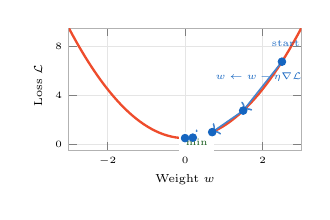
\begin{tikzpicture}[scale=0.7]
  \begin{axis}[
    width=5.8cm,height=3.8cm,
    xlabel={\fontsize{6pt}{7pt}\selectfont Weight $w$},
    ylabel={\fontsize{6pt}{7pt}\selectfont Loss $\mathcal{L}$},
    xlabel style={font=\fontsize{6pt}{7pt}\selectfont,yshift=2pt},
    ylabel style={font=\fontsize{6pt}{7pt}\selectfont,xshift=2pt},
    xmin=-3,xmax=3,ymin=-0.5,ymax=9.5,
    tick label style={font=\fontsize{5pt}{6pt}\selectfont},
    xtick={-2,0,2},ytick={0,4,8},
    axis line style={gray!60},
    grid=major,grid style={gray!20},
  ]
  \addplot[very thick,pytorchred,domain=-3:3,samples=60]{x^2+0.5};
  \addplot[only marks,mark=*,mark size=2pt,codeblue] coordinates{(2.5,6.75)(1.5,2.75)(0.7,0.99)(0.2,0.54)(0.0,0.5)};
  \draw[->,thick,codeblue!80] (axis cs:2.5,6.75)--(axis cs:1.5,2.75);
  \draw[->,thick,codeblue!80] (axis cs:1.5,2.75)--(axis cs:0.7,0.99);
  \draw[->,thick,codeblue!80] (axis cs:0.7,0.99)--(axis cs:0.2,0.54);
  \node[font=\fontsize{5pt}{5pt}\selectfont,codeblue] at (axis cs:2.6,8.2) {start};
  \node[font=\fontsize{5pt}{5pt}\selectfont,mathgreen,fill=white] at (axis cs:0.3,0.2) {min};
  \node[font=\fontsize{5pt}{5pt}\selectfont,codeblue] at (axis cs:1.9,5.5) {$w\leftarrow w-\eta\nabla\mathcal{L}$};
  \end{axis}
\end{tikzpicture}
\end{center}

\mysubsec{Chain Rule --- Foundation of Backprop}

If $\mathcal{L}=f(g(h(\mathbf{x})))$:

\begin{tcolorbox}[mathbox]
\fontsize{8pt}{11pt}\selectfont
\vspace{-4pt}
\[
\frac{\partial\mathcal{L}}{\partial\mathbf{x}}=
\underbrace{\frac{\partial\mathcal{L}}{\partial f}}_{\text{loss}}\cdot
\underbrace{\frac{\partial f}{\partial g}}_{\text{L3}}\cdot
\underbrace{\frac{\partial g}{\partial h}}_{\text{L2}}\cdot
\underbrace{\frac{\partial h}{\partial\mathbf{x}}}_{\text{L1}}
\]
\vspace{-5pt}
\end{tcolorbox}

\mysubsec{Worked Example}

$y=3x^3+2x+1$, find $dy/dx$ at $x=4$:

{\fontsize{7.5pt}{10pt}\selectfont
$\dfrac{dy}{dx}=9x^2+2$ \qquad At $x{=}4$: $9(16)+2=\mathbf{146}$}

\begin{lstlisting}
x = torch.tensor(4.0, requires_grad=True)
y = 3*x**3 + 2*x + 1
y.backward()
print(x.grad)    # tensor(146.)
\end{lstlisting}

\mysubsec{Computation Graph}

\begin{center}
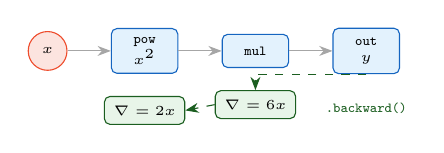
\begin{tikzpicture}[
  node distance=0.5cm and 0.55cm,
  op/.style={draw=codeblue,fill=defblue,rounded corners=2pt,minimum width=24pt,minimum height=12pt,font=\fontsize{5pt}{6pt}\selectfont,align=center},
  leaf/.style={draw=pytorchred,fill=pytorchred!15,circle,minimum size=14pt,font=\fontsize{5pt}{6pt}\selectfont\bfseries},
  grad/.style={draw=mathgreen,fill=tipgreen,rounded corners=2pt,minimum width=24pt,minimum height=10pt,font=\fontsize{4.5pt}{6pt}\selectfont},
  arr/.style={->,>=Stealth,thin,gray!70},
  garr/.style={->,>=Stealth,thin,dashed,mathgreen}
]
  \node[leaf] (x) {$x$};
  \node[op,right=of x] (sq) {\texttt{pow}\\$x^2$};
  \node[op,right=of sq] (mul) {\texttt{mul}};
  \node[op,right=of mul] (y) {\texttt{out}\\$y$};
  \draw[arr](x)--(sq);\draw[arr](sq)--(mul);\draw[arr](mul)--(y);
  \node[grad,below=0.28cm of sq] (gx) {$\nabla=2x$};
  \node[grad,below=0.28cm of mul] (gm) {$\nabla=6x$};
  \draw[garr](y.south)-|(gm.north);
  \draw[garr](gm.west)--(gx.east);
  \node[font=\fontsize{4pt}{5pt}\selectfont,mathgreen,below=7pt] at (y.south) {\texttt{.backward()}};
\end{tikzpicture}
\end{center}

\begin{lstlisting}
x = torch.tensor(3.0, requires_grad=True)
y = x ** 2
y.backward()
print(x.grad)     # 6.0  (= 2*3)
\end{lstlisting}

\begin{lstlisting}
# Stop tracking (inference)
with torch.no_grad():
    pred = model(x)
t.detach()   # new tensor, no grad history
\end{lstlisting}

\begin{tcolorbox}[warnbox,title=Sacred Training Loop Order]
\fontsize{7pt}{9pt}\selectfont
\textbf{1.} \texttt{pred=model(X)} \hfill forward\\
\textbf{2.} \texttt{loss=criterion(pred,y)} \hfill loss\\
\textbf{3.} \texttt{optimizer.zero\_grad()} \hfill CLEAR\\
\textbf{4.} \texttt{loss.backward()} \hfill backprop\\
\textbf{5.} \texttt{optimizer.step()} \hfill update
\end{tcolorbox}

\begin{tcolorbox}[tipbox,title=Why zero\_grad Matters]
\fontsize{7pt}{9pt}\selectfont
Gradients \textbf{accumulate} (add to \texttt{.grad}). Without clearing, batch 2's gradients pile on batch 1's --- updates are wrong from iteration 2 onward.
\end{tcolorbox}

\end{multicols}

%%%% PAGE 3 - LAYERS + ACTIVATIONS + LOSS %%%%
\newpage
\begin{multicols}{3}

\mysec{deepblue}{nn.MODULE --- THE BACKBONE}

\begin{tcolorbox}[defbox,title=Definition]
\fontsize{7pt}{9pt}\selectfont
\texttt{nn.Module} is the base class for all models. Every custom model \textbf{must} inherit from it. Implement: \texttt{\_\_init\_\_} (layers) and \texttt{forward} (data flow).
\end{tcolorbox}

\begin{lstlisting}
import torch.nn as nn

class MyNet(nn.Module):
    def __init__(self):
        super().__init__()   # ALWAYS first!
        self.fc1 = nn.Linear(784, 128)
        self.fc2 = nn.Linear(128, 10)
        self.relu = nn.ReLU()

    def forward(self, x):
        x = self.relu(self.fc1(x))
        return self.fc2(x)

model = MyNet()
\end{lstlisting}

\mysec{tealcolor}{KEY LAYERS --- MATH}

\mysubsec{nn.Linear --- Fully Connected}

\begin{tcolorbox}[mathbox]
\fontsize{9pt}{12pt}\selectfont
\vspace{-4pt}
\[
\mathbf{y}=\mathbf{x}\mathbf{W}^\top+\mathbf{b}
\]
\vspace{-6pt}
\end{tcolorbox}

$\mathbf{W}\in\mathbb{R}^{\text{out}\times\text{in}}$, $\mathbf{b}\in\mathbb{R}^{\text{out}}$

Params $=(\text{in}\times\text{out})+\text{out}$

\texttt{Linear(512,256)}: $512{\times}256+256=\mathbf{131{,}328}$

\mysubsec{Why Activations Are Needed}

\begin{tcolorbox}[tipbox,title=Key Insight]
\fontsize{7pt}{9pt}\selectfont
Without non-linearity: $\mathbf{W}_2(\mathbf{W}_1\mathbf{x})=(\mathbf{W}_2\mathbf{W}_1)\mathbf{x}$ --- stacking linear layers $\equiv$ one linear layer. Activations enable complex patterns.
\end{tcolorbox}

\mysubsec{ReLU}

\begin{tcolorbox}[mathbox]
\fontsize{8pt}{11pt}\selectfont
\vspace{-4pt}
\[
f(x)=\max(0,x),\quad f'(x)=\begin{cases}1&x>0\\0&x\le0\end{cases}
\]
\vspace{-5pt}
\end{tcolorbox}

\begin{center}
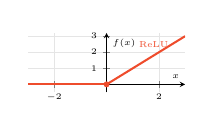
\begin{tikzpicture}[scale=0.62]
  \begin{axis}[
    width=4.8cm,height=2.8cm,
    xmin=-3,xmax=3,ymin=-0.5,ymax=3.2,
    xlabel={\fontsize{5pt}{6pt}\selectfont $x$},
    ylabel={\fontsize{5pt}{6pt}\selectfont $f(x)$},
    xlabel style={yshift=2pt},ylabel style={xshift=2pt},
    tick label style={font=\fontsize{5pt}{6pt}\selectfont},
    xtick={-2,0,2},ytick={0,1,2,3},
    grid=major,grid style={gray!20},axis lines=center,
  ]
  \addplot[very thick,pytorchred,domain=-3:0]{0};
  \addplot[very thick,pytorchred,domain=0:3]{x};
  \addplot[only marks,mark=*,mark size=1.5pt,pytorchred] coordinates{(0,0)};
  \node[font=\fontsize{5pt}{5pt}\selectfont,pytorchred] at (axis cs:1.8,2.5) {ReLU};
  \end{axis}
\end{tikzpicture}
\end{center}

\mysubsec{Sigmoid and Tanh}

\begin{tcolorbox}[mathbox]
\fontsize{7.5pt}{10pt}\selectfont
\vspace{-4pt}
\[
\sigma(x)=\frac{1}{1+e^{-x}}\in(0,1),\quad\sigma'=\sigma(1-\sigma)
\]
\[
\tanh(x)=\frac{e^x-e^{-x}}{e^x+e^{-x}}\in(-1,1)
\]
\vspace{-5pt}
\end{tcolorbox}

\begin{center}
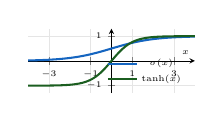
\begin{tikzpicture}[scale=0.62]
  \begin{axis}[
    width=5.0cm,height=2.9cm,
    xmin=-4,xmax=4,ymin=-1.3,ymax=1.3,
    xlabel={\fontsize{5pt}{6pt}\selectfont $x$},
    tick label style={font=\fontsize{5pt}{6pt}\selectfont},
    xlabel style={yshift=2pt},
    xtick={-3,-1,1,3},ytick={-1,0,1},
    grid=major,grid style={gray!20},
    axis lines=center,
    legend pos=south east,
    legend style={font=\fontsize{5pt}{6pt}\selectfont,draw=none,fill=none}
  ]
  \addplot[very thick,codeblue,domain=-4:4,samples=80]{1/(1+exp(-x))};
  \addlegendentry{$\sigma(x)$}
  \addplot[very thick,mathgreen,domain=-4:4,samples=80]{tanh(x)};
  \addlegendentry{$\tanh(x)$}
  \end{axis}
\end{tikzpicture}
\end{center}

\mysubsec{Softmax}

\begin{tcolorbox}[mathbox]
\fontsize{8pt}{11pt}\selectfont
\vspace{-4pt}
\[
\text{softmax}(\mathbf{z})_i=\frac{e^{z_i}}{\sum_{j=1}^{K}e^{z_j}},\quad\sum_i p_i=1
\]
\vspace{-5pt}
\end{tcolorbox}

\mysubsec{Activation Summary}

{\fontsize{6.5pt}{8pt}\selectfont
\begin{tabular}{@{}llll@{}}
\toprule
\textbf{Name}&\textbf{Range}&\textbf{Use}&\textbf{Vanish?}\\
\midrule
ReLU&$[0,\infty)$&Hidden&No\\
Sigmoid&$(0,1)$&Binary out&Yes\\
Tanh&$(-1,1)$&Hidden,RNN&Mild\\
Softmax&$(0,1)^K$&Multi-class&---\\
\bottomrule
\end{tabular}}

\mysec{pytorchred}{LOSS FUNCTIONS}

\mysubsec{MSE --- Regression}

\begin{tcolorbox}[mathbox]
\fontsize{8pt}{11pt}\selectfont
\vspace{-4pt}
\[
\mathcal{L}_{\text{MSE}}=\frac{1}{n}\sum_{i=1}^{n}(\hat{y}_i-y_i)^2
\]
\vspace{-5pt}
\end{tcolorbox}

\texttt{nn.MSELoss()} --- linear output.

\mysubsec{Binary Cross Entropy}

\begin{tcolorbox}[mathbox]
\fontsize{7.5pt}{10pt}\selectfont
\vspace{-4pt}
\[
\mathcal{L}_{\text{BCE}}=-\frac{1}{n}\sum_i\left[y_i\log\hat{y}_i+(1{-}y_i)\log(1{-}\hat{y}_i)\right]
\]
\vspace{-5pt}
\end{tcolorbox}

\begin{tcolorbox}[warnbox,title=Use BCEWithLogitsLoss]
\fontsize{7pt}{9pt}\selectfont
Applies sigmoid internally. More numerically stable. Never use \texttt{BCELoss} + manual sigmoid.
\end{tcolorbox}

\mysubsec{Cross Entropy --- Multiclass}

\begin{tcolorbox}[mathbox]
\fontsize{8pt}{11pt}\selectfont
\vspace{-4pt}
\[
\mathcal{L}_{\text{CE}}=-\frac{1}{n}\sum_i\sum_j y_{ij}\log\hat{y}_{ij}
\]
\vspace{-5pt}
\end{tcolorbox}

\begin{tcolorbox}[warnbox,title=CRITICAL --- No Softmax Before CE]
\fontsize{7pt}{9pt}\selectfont
\texttt{CrossEntropyLoss}=LogSoftmax+NLLLoss. Passing softmax outputs applies softmax twice --- \textbf{silent} wrong results.
\end{tcolorbox}

\mysubsec{Loss Selection --- Memorise}

{\fontsize{6.5pt}{8pt}\selectfont
\begin{tabular}{@{}lll@{}}
\toprule
\textbf{Task}&\textbf{Loss}&\textbf{Output}\\
\midrule
Regression&\texttt{MSELoss}&linear\\
Binary cls&\texttt{BCEWithLogitsLoss}&linear\\
Multi-class&\texttt{CrossEntropyLoss}&linear\\
\bottomrule
\end{tabular}}

\end{multicols}

%%%% PAGE 4 - OPTIMIZERS + BACKPROP + BATCHNORM + DROPOUT %%%%
\newpage
\begin{multicols}{3}

\mysec{accentpurple}{BACKPROPAGATION --- VISUAL}

\begin{center}
\begin{tikzpicture}[
  scale=0.65,
  nd/.style={circle,draw=codeblue,fill=defblue,minimum size=15pt,font=\fontsize{5pt}{6pt}\selectfont},
  on/.style={circle,draw=pytorchred,fill=pytorchred!15,minimum size=15pt,font=\fontsize{5pt}{6pt}\selectfont},
  hn/.style={circle,draw=mathgreen,fill=tipgreen,minimum size=15pt,font=\fontsize{5pt}{6pt}\selectfont},
  arr/.style={->,>=Stealth,gray!60,thin},
  barr/.style={->,>=Stealth,pytorchred!80,dashed,thin},
]
  \foreach \y/\l in {1/$x_1$,0/$x_2$,-1/$x_3$}{\node[nd](i\y) at (0,\y){\l};}
  \foreach \y/\l in {1.2/$h_1$,0/$h_2$,-1.2/$h_3$}{\node[hn](h\y) at (2.2,\y){\l};}
  \foreach \y/\l in {0.5/$o_1$,-0.5/$o_2$}{\node[on](o\y) at (4.2,\y){\l};}
  \foreach \i in {1,0,-1}{\foreach \h in {1.2,0,-1.2}{\draw[arr](i\i)--(h\h);}}
  \foreach \h in {1.2,0,-1.2}{\foreach \o in {0.5,-0.5}{\draw[arr](h\h)--(o\o);}}
  \node[draw=pytorchred,fill=pytorchred!20,rounded corners=2pt,minimum width=18pt,minimum height=12pt,font=\fontsize{5pt}{6pt}\selectfont](loss) at (5.8,0){$\mathcal{L}$};
  \draw[arr,pytorchred](o0.5)--(loss);\draw[arr,pytorchred](o-0.5)--(loss);
  \draw[barr](loss.south)..controls(5.0,-1.6)and(3.5,-1.9)..(h-1.2.south);
  \draw[barr](h-1.2.south)..controls(1.5,-2.0)and(0.5,-1.7)..(i-1.south);
  \node[font=\fontsize{5pt}{6pt}\selectfont,codeblue] at (0,-1.8) {Input};
  \node[font=\fontsize{5pt}{6pt}\selectfont,mathgreen] at (2.2,-1.8) {Hidden};
  \node[font=\fontsize{4.5pt}{5pt}\selectfont,gray] at (1.1,1.8) {\textit{forward}$\rightarrow$};
  \node[font=\fontsize{4.5pt}{5pt}\selectfont,pytorchred!80] at (2.2,-2.35) {\textit{backward}$\leftarrow$};
\end{tikzpicture}
\end{center}

{\fontsize{6.5pt}{8pt}\selectfont
\textbf{Forward}: data flows input $\to$ output, graph built.\\
\textbf{Backward}: gradients flow output $\to$ input via chain rule.\\
Each weight: $w\leftarrow w-\eta\,\dfrac{\partial\mathcal{L}}{\partial w}$}

\mysec{deepblue}{OPTIMIZERS}

\mysubsec{SGD}

\begin{tcolorbox}[mathbox]
\fontsize{8pt}{11pt}\selectfont
\vspace{-4pt}
\[
\mathbf{w}^{(t+1)}=\mathbf{w}^{(t)}-\eta g_t
\]
With momentum: $v_t=\beta v_{t-1}+(1-\beta)g_t$
\vspace{-3pt}
\end{tcolorbox}

\begin{lstlisting}
torch.optim.SGD(model.parameters(), lr=0.01)
torch.optim.SGD(model.parameters(), lr=0.01, momentum=0.9)
\end{lstlisting}

\mysubsec{Adam --- Adaptive Moment Estimation}

\begin{tcolorbox}[mathbox,title=Adam Equations]
\fontsize{7.5pt}{10pt}\selectfont
\vspace{-2pt}
\begin{align*}
m_t&=\beta_1 m_{t-1}+(1-\beta_1)g_t\quad\text{(1st moment)}\\
v_t&=\beta_2 v_{t-1}+(1-\beta_2)g_t^2\quad\text{(2nd moment)}\\
\hat{m}_t&=\frac{m_t}{1-\beta_1^t},\quad\hat{v}_t=\frac{v_t}{1-\beta_2^t}\quad\text{(bias corr)}\\
\mathbf{w}&\leftarrow\mathbf{w}-\eta\frac{\hat{m}_t}{\sqrt{\hat{v}_t}+\varepsilon}
\end{align*}
\vspace{-6pt}
\end{tcolorbox}

Defaults: $\beta_1{=}0.9$, $\beta_2{=}0.999$, $\varepsilon{=}10^{-8}$

\begin{lstlisting}
torch.optim.Adam(model.parameters(), lr=1e-3)
\end{lstlisting}

{\fontsize{6.5pt}{8pt}\selectfont
\begin{tabular}{@{}lll@{}}
\toprule
\textbf{Optimizer}&\textbf{Best For}&\textbf{lr}\\
\midrule
SGD&Vision tasks&0.01\\
SGD+momentum&Faster conv.&0.01\\
Adam&Default choice&0.001\\
AdamW&Transformers&0.001\\
\bottomrule
\end{tabular}}

\mysec{tealcolor}{BATCH NORMALISATION}

\begin{tcolorbox}[mathbox]
\fontsize{8pt}{11pt}\selectfont
\vspace{-4pt}
\[
\hat{x}_i=\frac{x_i-\mu_\mathcal{B}}{\sqrt{\sigma^2_\mathcal{B}+\varepsilon}},\qquad y_i=\gamma\hat{x}_i+\beta
\]
\vspace{-5pt}
\end{tcolorbox}

$\gamma,\beta$ are \textit{learned}. During \texttt{eval()}: uses running stats.

\begin{lstlisting}
nn.BatchNorm1d(num_features)  # after Linear
nn.BatchNorm2d(num_channels)  # after Conv2d
\end{lstlisting}

\textbf{Benefits:} faster training, higher LR tolerance, mild regularisation.

\mysec{pytorchred}{DROPOUT}

\begin{tcolorbox}[mathbox]
\fontsize{8pt}{11pt}\selectfont
\vspace{-4pt}
\[
\tilde{h}_i=\frac{h_i\cdot m_i}{1-p},\quad m_i\sim\text{Bernoulli}(1-p)
\]
\vspace{-5pt}
\end{tcolorbox}

Randomly zeros neurons with prob $p$ during training.

\begin{lstlisting}
nn.Dropout(p=0.5)    # 50% zeroed (train)
# eval(): automatically disabled
\end{lstlisting}

\begin{center}
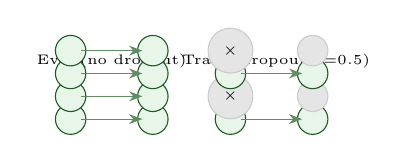
\begin{tikzpicture}[scale=0.58,font=\tiny]
  \node[font=\fontsize{5.5pt}{7pt}\selectfont,above] at (0.9,0.9) {Eval (no dropout)};
  \foreach \y in {0,0.5,1.0,1.5}{
    \node[circle,draw=mathgreen,fill=tipgreen,minimum size=11pt] at (0,\y){};
    \node[circle,draw=mathgreen,fill=tipgreen,minimum size=11pt] at (1.8,\y){};
    \draw[->,>=Stealth,mathgreen!70,thin](0.23,\y)--(1.57,\y);
  }
  \node[font=\fontsize{5.5pt}{7pt}\selectfont,above] at (4.5,0.9) {Train (dropout $p{=}0.5$)};
  \foreach \y/\drop in {0/0,0.5/1,1.0/0,1.5/1}{
    \ifnum\drop=0
      \node[circle,draw=mathgreen,fill=tipgreen,minimum size=11pt] at (3.5,\y){};
      \node[circle,draw=mathgreen,fill=tipgreen,minimum size=11pt] at (5.3,\y){};
      \draw[->,>=Stealth,mathgreen!70,thin](3.73,\y)--(5.07,\y);
    \else
      \node[circle,draw=gray!40,fill=gray!20,minimum size=11pt,font=\fontsize{5pt}{5pt}\selectfont] at (3.5,\y){$\times$};
      \node[circle,draw=gray!40,fill=gray!20,minimum size=11pt] at (5.3,\y){};
    \fi
  }
\end{tikzpicture}
\end{center}

\mysec{accentpurple}{nn.Sequential}

\begin{lstlisting}
model = nn.Sequential(
    nn.Linear(784, 256),
    nn.BatchNorm1d(256),
    nn.ReLU(),
    nn.Dropout(0.3),
    nn.Linear(256, 128),
    nn.ReLU(),
    nn.Linear(128, 10)
)
\end{lstlisting}

\begin{tcolorbox}[tipbox,title=Sequential vs Module]
\fontsize{7pt}{9pt}\selectfont
\texttt{Sequential}: simple linear stacks.\\
\texttt{nn.Module}: skip connections, multiple inputs/outputs, custom logic.
\end{tcolorbox}

\end{multicols}

%%%% PAGE 5 - DATASETS + CNN + COMPLETE PIPELINE %%%%
\newpage
\begin{multicols}{3}

\mysec{tealcolor}{DATASETS \& DATALOADERS}

\begin{tcolorbox}[defbox,title=Definition]
\fontsize{7pt}{9pt}\selectfont
\textbf{Dataset}: Abstract class. Must implement \texttt{\_\_len\_\_} and \texttt{\_\_getitem\_\_}.\\
\textbf{DataLoader}: Wraps Dataset; batching, shuffling, parallel loading.
\end{tcolorbox}

\begin{lstlisting}
from torch.utils.data import Dataset, DataLoader

class MyDataset(Dataset):
    def __init__(self, X, y):
        self.X, self.y = X, y

    def __len__(self):
        return len(self.X)

    def __getitem__(self, idx):
        return self.X[idx], self.y[idx]

ds = MyDataset(X_tensor, y_tensor)
dl = DataLoader(ds, batch_size=32, shuffle=True)
\end{lstlisting}

{\fontsize{6.5pt}{8pt}\selectfont
\begin{tabular}{@{}ll@{}}
\toprule
\textbf{Param}&\textbf{Meaning}\\
\midrule
\texttt{batch\_size}&Samples per iteration\\
\texttt{shuffle=True}&Randomise each epoch\\
\texttt{num\_workers}&Parallel loading threads\\
\texttt{drop\_last}&Drop final small batch\\
\bottomrule
\end{tabular}}

\mysec{pytorchred}{MODEL MODES}

\begin{tcolorbox}[warnbox,title=Always Switch Modes]
\fontsize{7pt}{9pt}\selectfont
\textbf{model.train()}: Dropout active, BN uses batch stats.\\
\textbf{model.eval()}: Dropout off, BN uses running stats.\\
Forgetting this \textbf{silently} degrades performance!
\end{tcolorbox}

\begin{lstlisting}
model.train()
for X, y in train_dl:
    ...   # training loop

model.eval()
with torch.no_grad():
    for X, y in val_dl:
        pred = model(X)
\end{lstlisting}

\mysec{deepblue}{CONVOLUTIONAL LAYERS (CNN)}

\mysubsec{Output Spatial Size}

\begin{tcolorbox}[mathbox]
\fontsize{8pt}{11pt}\selectfont
\vspace{-4pt}
\[
H_{out}=\left\lfloor\frac{H_{in}+2P-K}{S}\right\rfloor+1
\]
\vspace{-5pt}
\end{tcolorbox}

$P$=padding, $K$=kernel, $S$=stride. Same for $W_{out}$.

\mysubsec{Parameter Count}

\begin{tcolorbox}[mathbox]
\fontsize{8pt}{11pt}\selectfont
\vspace{-4pt}
\[
\text{params}=C_{out}\times(C_{in}\times K^2+1)
\]
\vspace{-5pt}
\end{tcolorbox}

\texttt{Conv2d(3,64,3)}: $64{\times}(3{\times}9+1)=\mathbf{1{,}792}$

\begin{lstlisting}
nn.Conv2d(3, 64, kernel_size=3, padding=1)
# padding=1 with kernel=3 -> same spatial size
nn.MaxPool2d(kernel_size=2, stride=2)
# halves both H and W
\end{lstlisting}

\begin{center}
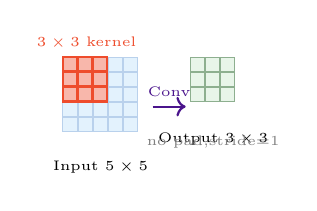
\begin{tikzpicture}[scale=0.6,font=\tiny]
  \foreach \r in {0,...,4}{
    \foreach \c in {0,...,4}{
      \fill[defblue,draw=codeblue!30,line width=0.3pt](\c*0.32,-\r*0.32)rectangle(\c*0.32+0.30,-\r*0.32+0.30);
    }
  }
  \foreach \r in {0,1,2}{
    \foreach \c in {0,1,2}{
      \fill[pytorchred!40,draw=pytorchred,line width=0.8pt](\c*0.32,-\r*0.32)rectangle(\c*0.32+0.30,-\r*0.32+0.30);
    }
  }
  \node[below,font=\fontsize{5pt}{6pt}\selectfont] at (0.8,-1.7) {Input $5\times5$};
  \node[font=\fontsize{5pt}{5pt}\selectfont,pytorchred] at (0.5,0.6) {$3\times3$ kernel};
  \draw[->,thick,accentpurple](1.9,-0.75)--node[above,font=\fontsize{5pt}{6pt}\selectfont,accentpurple]{Conv}(2.6,-0.75);
  \foreach \r in {0,...,2}{
    \foreach \c in {0,...,2}{
      \fill[tipgreen,draw=mathgreen!50,line width=0.3pt](2.7+\c*0.32,-\r*0.32)rectangle(2.7+\c*0.32+0.30,-\r*0.32+0.30);
    }
  }
  \node[below,font=\fontsize{5pt}{6pt}\selectfont] at (3.18,-1.1) {Output $3\times3$};
  \node[font=\fontsize{4.5pt}{5pt}\selectfont,gray] at (3.18,-1.5) {no pad,stride=1};
\end{tikzpicture}
\end{center}

\mysec{accentpurple}{SAVING \& LOADING}

\begin{lstlisting}
torch.save(model.state_dict(), "model.pth")

model = MyNet()
model.load_state_dict(torch.load("model.pth"))
model.eval()
\end{lstlisting}

\begin{tcolorbox}[tipbox,title=Why state\_dict?]
\fontsize{7pt}{9pt}\selectfont
Saves only parameter tensors. Portable across codebases. Saving whole model pickles the class --- breaks on refactor or rename.
\end{tcolorbox}

\mysec{tealcolor}{COMPLETE TRAINING PIPELINE}

\begin{lstlisting}
import torch, torch.nn as nn
from torch.utils.data import DataLoader, TensorDataset

# Data
X = torch.randn(1000, 20)
y = torch.randint(0, 3, (1000,))
ds = TensorDataset(X, y)
train_ds, val_ds = torch.utils.data.random_split(
    ds, [800, 200])
train_dl = DataLoader(train_ds, batch_size=32, shuffle=True)
val_dl   = DataLoader(val_ds, batch_size=32)

# Model
class Net(nn.Module):
    def __init__(self):
        super().__init__()
        self.net = nn.Sequential(
            nn.Linear(20,64), nn.ReLU(),
            nn.Linear(64,32), nn.ReLU(),
            nn.Linear(32,3))
    def forward(self, x): return self.net(x)

device = "cuda" if torch.cuda.is_available() else "cpu"
model  = Net().to(device)
crit   = nn.CrossEntropyLoss()
optim  = torch.optim.Adam(model.parameters(), lr=1e-3)

# Loop
for epoch in range(10):
    model.train(); tloss = 0
    for Xb,yb in train_dl:
        Xb,yb = Xb.to(device), yb.to(device)
        loss = crit(model(Xb), yb)
        optim.zero_grad(); loss.backward()
        optim.step(); tloss += loss.item()
    model.eval(); correct = 0
    with torch.no_grad():
        for Xb,yb in val_dl:
            Xb,yb = Xb.to(device), yb.to(device)
            correct += (model(Xb).argmax(1)==yb).sum().item()
    print(f"Ep{epoch+1} Loss:{tloss/len(train_dl):.3f} Acc:{correct/200:.3f}")

torch.save(model.state_dict(), "model.pth")
\end{lstlisting}

\end{multicols}

%%%% PAGE 6 - PRACTICE + SOLUTIONS + TIPS %%%%
\newpage
\begin{multicols}{3}

\mysec{pytorchred}{PRACTICE QUESTIONS}

\mysubsec{Section A --- Conceptual}

\begin{enumerate}[label=\textcolor{pytorchred}{\textbf{Q\arabic*.}},leftmargin=18pt]
\fontsize{6.8pt}{9pt}\selectfont
\item Explain dynamic vs static computation graphs. Why does PyTorch's approach aid debugging?
\item What are the \textbf{three} core tensor attributes? Describe each.
\item Why must \texttt{optimizer.zero\_grad()} be called before \texttt{loss.backward()}?
\item Why should you \textit{never} apply softmax before \texttt{nn.CrossEntropyLoss()}?
\item Difference between \texttt{model.train()} and \texttt{model.eval()}? Name 2 affected layers.
\item Write chain rule for $\mathcal{L}=f(g(h(\mathbf{x})))$ w.r.t.\ $\mathbf{x}$.
\item What does \texttt{requires\_grad=True} do? When is the graph built?
\end{enumerate}

\mysubsec{Section B --- Shape Tracing}

\begin{enumerate}[label=\textcolor{codeblue}{\textbf{Q\arabic*.}},leftmargin=18pt,start=8]
\fontsize{6.8pt}{9pt}\selectfont
\item \texttt{t=randn(4,3,28,28)}. Shapes after: \texttt{view(4,-1)}, \texttt{permute(0,2,3,1)}, \texttt{[:,0,:,:]}?
\item \texttt{a=randn(32,64)}, \texttt{b=randn(64,128)}. Shape of \texttt{a @ b}?
\item \texttt{t=randn(8,16)}, shape of \texttt{t.unsqueeze(0).unsqueeze(2)}?
\item \texttt{t=randn(3,1,5)}, shape of \texttt{t.squeeze()}?
\item Shape $(100,)\to(100,1)$. What single call?
\end{enumerate}

\mysubsec{Section C --- Debug the Code}

\begin{enumerate}[label=\textcolor{warnorange}{\textbf{Q\arabic*.}},leftmargin=18pt,start=13]
\fontsize{6.8pt}{9pt}\selectfont
\item User wants matmul but writes \texttt{result=x*y} for $(10,5)$ matrices.
\item \texttt{model} on CPU, \texttt{x=randn(32,784).to("cuda")}, then \texttt{model(x)}.
\item Training loop missing one line --- gradients accumulate across batches.
\item \texttt{probs=Softmax(logits)}, then \texttt{loss=CrossEntropyLoss(probs,y)}.
\item Eval loop has no \texttt{torch.no\_grad()} wrapper.
\end{enumerate}

\mysubsec{Section D --- Math Questions}

\begin{enumerate}[label=\textcolor{mathgreen}{\textbf{Q\arabic*.}},leftmargin=18pt,start=18]
\fontsize{6.8pt}{9pt}\selectfont
\item $y=3x^3+2x+1$: find $dy/dx$ at $x{=}4$. What does \texttt{x.grad} print?
\item \texttt{Linear(512,256)}: how many trainable parameters?
\item \texttt{Conv2d(3,64,3)}: how many parameters?
\item PIL image $(H{=}256,W{=}256,C{=}3)$: what converts to PyTorch format?
\item Output $(32,10)$: write 2 lines for predictions and accuracy vs \texttt{y} shape $(32,)$.
\end{enumerate}

\columnbreak

\mysec{deepblue}{SOLUTIONS}

\mysubsec{Section A}

{\fontsize{6.5pt}{8.5pt}\selectfont
\textbf{A1.} Static graphs compile before execution (fixed). Dynamic build during execution --- normal Python control flow, \texttt{print()}, \texttt{pdb} all work directly.

\textbf{A2.} \texttt{dtype} (data type), \texttt{shape} (dimensions), \texttt{device} (cpu/cuda/mps).

\textbf{A3.} Gradients \textit{accumulate} (add to \texttt{.grad}). Without clearing, batches 2+ have wrong accumulated gradients baked into updates.

\textbf{A4.} \texttt{CrossEntropyLoss} applies log-softmax internally. Passing softmax outputs doubles it --- wrong loss, no error thrown. Silent bug.

\textbf{A5.} \texttt{train()}: Dropout active, BN uses batch stats. \texttt{eval()}: Dropout off, BN uses running stats accumulated during training.

\textbf{A6.} $\dfrac{\partial\mathcal{L}}{\partial\mathbf{x}}=\dfrac{\partial\mathcal{L}}{\partial f}\cdot\dfrac{\partial f}{\partial g}\cdot\dfrac{\partial g}{\partial h}\cdot\dfrac{\partial h}{\partial\mathbf{x}}$

\textbf{A7.} Tells PyTorch to track all ops on this tensor in a DAG. Graph built \textit{dynamically} during forward pass. \texttt{.backward()} traverses in reverse.}

\mysubsec{Section B}

{\fontsize{6.5pt}{8.5pt}\selectfont
\textbf{B8.} \texttt{view(4,-1)}: $(4,2352)$ since $3\times28^2{=}2352$; \texttt{permute(0,2,3,1)}: $(4,28,28,3)$; \texttt{[:,0,:,:]}: $(4,28,28)$

\textbf{B9.} $(32,128)$ --- inner dims match; outer dims form result.

\textbf{B10.} $(8,16)\to(1,8,16)\to\mathbf{(1,8,1,16)}$

\textbf{B11.} $(3,5)$ --- size-1 middle dim removed.

\textbf{B12.} \texttt{t.unsqueeze(1)} or \texttt{t.reshape(100,1)}}

\mysubsec{Section C}

{\fontsize{6.5pt}{8.5pt}\selectfont
\textbf{C13.} \texttt{x*y}=element-wise. For matmul: \texttt{x @ y} or \texttt{torch.matmul(x,y)}.

\textbf{C14.} Model is on CPU, data on CUDA. Fix: \texttt{model.to("cuda")} before \texttt{model(x)}.

\textbf{C15.} Missing \texttt{optimizer.zero\_grad()} before \texttt{loss.backward()}.

\textbf{C16.} Softmax before CrossEntropyLoss --- double applies. Pass raw logits.

\textbf{C17.} Wrap with \texttt{with torch.no\_grad():} --- saves memory, faster.}

\mysubsec{Section D}

{\fontsize{6.5pt}{8.5pt}\selectfont
\textbf{D18.} $dy/dx=9x^2+2$. At $x{=}4$: $\mathbf{146}$. \texttt{x.grad = tensor(146.)}

\textbf{D19.} $(512\times256)+256=\mathbf{131{,}328}$

\textbf{D20.} $64\times(3\times9+1)=64\times28=\mathbf{1{,}792}$

\textbf{D21.} \texttt{tensor.permute(2,0,1)}: $(H,W,C)\to(C,H,W)$

\textbf{D22.} \texttt{preds=output.argmax(dim=1)}\\
\phantom{\textbf{D22.}}\texttt{acc=(preds==y).float().mean().item()}}

\mysec{tealcolor}{TIPS \& TRICKS --- LOCK IN}

{\fontsize{6.5pt}{8.5pt}\selectfont
\begin{enumerate}[label=\textcolor{pytorchred}{\textbf{\arabic*.}},leftmargin=14pt]
\item \textbf{Shape debug first.} Print \texttt{t.shape} at every step. 90\% of errors are shape mismatches.
\item \textbf{Always \texttt{loss.item()}} to log --- avoids accumulating GPU tensors.
\item \textbf{Normalise inputs} to $[-1,1]$: use $(x-\mu)/\sigma$.
\item \textbf{Default: Adam, lr=1e-3.} Too high: loss explodes. Too low: stuck.
\item \textbf{Set seed:} \texttt{torch.manual\_seed(42)} for reproducibility.
\item \textbf{No softmax before CrossEntropyLoss.} Silent error, not a crash.
\item \textbf{model.parameters()} for optimizer; \textbf{state\_dict()} for saving.
\item \textbf{no\_grad() always} during inference --- faster, less memory.
\item \textbf{Classification predictions:} \texttt{output.argmax(dim=1)}.
\item \textbf{Start small.} Debug on 10 samples, then scale up.
\end{enumerate}}

\mysec{accentpurple}{QUICK REFERENCE}

{\fontsize{6.3pt}{8pt}\selectfont
\renewcommand{\arraystretch}{1.2}
\begin{tabular}{@{}ll@{}}
\toprule
\textbf{Concept}&\textbf{Syntax}\\
\midrule
Matrix multiply&\texttt{A @ B}\\
Enable gradient&\texttt{requires\_grad=True}\\
Backward pass&\texttt{loss.backward()}\\
Zero gradients&\texttt{optimizer.zero\_grad()}\\
Weight update&\texttt{optimizer.step()}\\
Stop gradients&\texttt{torch.no\_grad()}\\
Move to GPU&\texttt{tensor.to(device)}\\
Predictions&\texttt{out.argmax(dim=1)}\\
Save model&\texttt{torch.save(m.state\_dict(),...)}\\
Train mode&\texttt{model.train()}\\
Eval mode&\texttt{model.eval()}\\
\bottomrule
\end{tabular}}

\begin{tcolorbox}[warnbox,title=The Sacred 5-Step Training Loop]
\fontsize{7pt}{9pt}\selectfont
\textbf{1.} \texttt{pred=model(X)} \hfill forward\\
\textbf{2.} \texttt{loss=crit(pred,y)} \hfill loss\\
\textbf{3.} \texttt{optimizer.zero\_grad()} \hfill clear grads\\
\textbf{4.} \texttt{loss.backward()} \hfill backprop\\
\textbf{5.} \texttt{optimizer.step()} \hfill update weights
\end{tcolorbox}

\end{multicols}

\end{document}
